\documentclass[10pt]{beamer}
\usepackage{tcolorbox}
%\usepackage{float}
%\usepackage{tikz}    
\usepackage{amssymb}
\usetheme[progressbar=frametitle]{metropolis}
\usepackage{appendixnumberbeamer}
\usepackage[normalem]{ulem}
%\usepackage{booktabs}
%\usepackage[scale=2]{ccicons}
\usepackage[utf8]{inputenc}
%\usepackage{soul}
%\usepackage{pgfplots}
%\usepgfplotslibrary{dateplot}
 \usepackage{relsize}
%\usepackage{xspace}
\usepackage{graphicx}
% \usepackage{pifont}
\usefonttheme{professionalfonts}
%\usepackage{times}
\usepackage{amsmath}
\usepackage{verbatim}
\usepackage[utf8]{inputenc}
%\usepackage{tikzcd}

\usepackage{tikz}
\usetikzlibrary{matrix}

\newcommand{\themename}{\textbf{\textsc{metropolis}}\xspace}

\everymath{\displaystyle}

%\uselanguage{Spanish}
%\languagepath{Spanish}



%\usepackage[all,cmtip]{xy}
\usepackage{turnstile}


%\usepackage{tikz}
%\newcommand*\circled[1]{\tikz[baseline=(char.base)]{
 

%\newtheorem{theorem}{Theorem}
%\newtheorem{lemma}{Lemma}
\newtheorem{remark}{Remark}

\title{Cutting cuts}
\subtitle{Cut down to 10 minutes.}
\author{Alakh Dhruv Chopra and Guillermo (Billy) Mosse}
\institute{Chennai Mathematical Institute and Universidad de Buenos Aires}

\subject{Ordinal Analysis}
\usepackage{stackengine}

%\newcommand\letvdash[1]{\mathrel{
%  \stackengine{1ex}{\vdash}{\;\;\scriptscriptstyle#1}{O}{c}{F}{T}{L}}}
%\stackMath

%\newcommand\letvudash[1]{\mathrel{
 % \stackengine{.4ex}{\vdash}{\;\;\scriptscriptstyle#1}{U}{c}{F}{T}{L}}}

\newcommand\infsint[2]{\mathrel{
  \stackengine{1ex}{\vdash}{\;\;\scriptscriptstyle#1}{O}{c}{F}{T}{L}}
\mathrel{
  \stackengine{.4ex}{\vdash}{\;\;\scriptscriptstyle#2}{U}{c}{F}{T}{L}}  
  }
\stackMath


\def\sint{\vdash}
\def\sem{\vDash}

\makeatletter
\newcommand*\bigcdot{\mathpalette\bigcdot@{.5}}
\newcommand*\bigcdot@[2]{\mathbin{\vcenter{\hbox{\scalebox{#2}{$\m@th#1\bullet$}}}}}

% TODO Fix with input from Pohlers
\newcommand{\sintcons}[2]{\;\sststile{#2}{#1}\!}

\def\fomega{{\omega}^{\bigcdot}}
\usepackage{relsize}

\begin{document}


\maketitle

%Las preguntas deberían motivar lo que decimos, pero no abusar.
%O sea, no definir cosas en desorden solamente para arreglarlo con una pregunta.

%Hey guys and girls. As the title of the presentation suggests, [CLICK]	
\begin{frame}{What we want to prove}

% We want to talk about a general cut elimination theorem.

%So Professor Pohlers proved you today the Basic Elimination Lemma.
% It says that if you have a derivation of a set of formulas \Delta
% that uses the cut rule $\rho+1$ times then you can get a derivation
% with one less cut rank, but you pay the price of having a longer derivation.

\begin{lemma}{(Basic Elimination Lemma)}
If $\sintcons{\alpha}{\rho+1}\Delta$ then $\sintcons{\omega^\alpha}{\rho} \Delta$.
\end{lemma}

% By applying it iteratively you can get cut-free derivations of pseudo \Pi_1^1 sentences and that lets you find the truth complexity of a formula and actually bound it by $\varepsilon_0$ [CLICK]

\pause

\begin{lemma}{(Generalized Elimination Lemma)}
If $\sintcons{\alpha}{\beta+\omega^\rho} \Delta$ then $\sintcons{\varphi_\rho(\alpha)}{\beta} \Delta$.
\end{lemma}

% We now want to prove the following lemma, which is slighly more general than the previous one.

% QUES (ALAKH): But where did the omega come from? Aren't the ranks of formulas finite?
% ANS (BILLY): of course, this happens in the systems professor Pohlers presented, but there are other systems, like ATR_0, where you can have formulas of infinite complexity and there this lemma applies.

% OK, so you might be wondering what are those $\phi$ functions over there. They are called the Veblen functions. Let's talk a little bit about them. [CLICK]
\end{frame}

\begin{frame}{Veblen functions (defined inductively)}
\begin{figure}
\centering
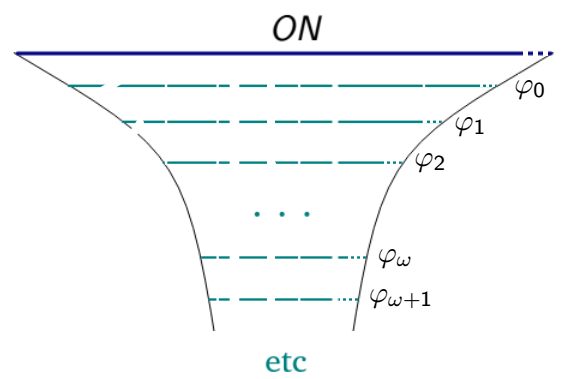
\includegraphics[scale=0.4]{veblen.png}
\caption{The range (image) of the first Veblen functions. Not to scale.}
\end{figure}

\begin{itemize}
	\item Zero ordinal: $\varphi_0(\alpha) := \omega^\alpha$
	%\item Successor ordinals $\rho + 1$: $\varphi_{\rho+1}(\alpha) := Enum\mathlarger{\mathlarger{(}}FIX\mathlarger{(}\varphi_\rho\mathlarger{)}\mathlarger{\mathlarger{)}}(\alpha)$
	\item Successor ordinals $\rho + 1$: $\varphi_{\rho+1}(\alpha) := Enum(FIX(\varphi_\rho), \alpha)$
	\item Limit ordinals $\lambda$: $\varphi_{\lambda}(\alpha) := Enum\mathlarger{(}\cap_{\rho < \lambda} FIX(\varphi(\rho)),\alpha\mathlarger{)}$
\end{itemize}

%The Veblen functions are functions on ordinals defined inductively, $\phi_0$ is just exponentiation on base \omega. As we are dealing with ordinals the inductive definition must be given for both successor ordinals and limit ordinals.

%For successor ordinals, you define the function as the enumeration of the fixed points of the previous functions

%And for limit ordinals we want to do something similar, but in this case there is no "previous" function, so you just take the enumeration of the common fixed points of all the previous ordinals.

% QUES (ALAKH): Isn´t it very similar to diagonalization
% ANS (BILLY): It's exactly a dioagnilzation! Very good, Alakh, you are paying attention. [CLICK]

\pause

%One slight remark is that by construction, the range of a veblen function is always a subset of the fixed points of each previous function. Just keep that in mind!
\textbf{Remark}: If $\rho_1 < \rho_2$ then $\varphi_{\rho_2}$ enumerates a subset of fixed points of $\varphi_{\rho_1}$

\end{frame}

\begin{frame}{Proof (1/5)}


We want to prove that:
$$
\sintcons{\alpha}{\beta+\omega^\rho} \Delta \text{ implies }
\sintcons{\phi_\rho(\alpha)}{\beta} \Delta
$$
\pause

% Now we get to the proof of the main lemma, where we remove a factor of omega to the rho from the cut rank at the expense of increasing the length of the proof with a veblen function. 

% So, what's the obvious thing to do in such a proof? [CLICK]
We induct on $\rho$.
\pause

% The base case is when rho is equal to 0. This case simply reduces to an instance of the basic elimination lemma.
For $\rho = 0$, we have $\sintcons{\alpha}{\beta + \omega^0} \Delta \equiv \sintcons{\alpha}{\beta +1} \Delta$.
By the Basic Elimination Lemma, we get
$\sintcons{\omega^\alpha}{\beta}\Delta
\equiv \sintcons{\varphi_0(\alpha)}{\beta} \Delta$.

% so we get the result for free.

% QUES (ALAKH): But doesn't the that theorem only deal with finite cut ranks? How can you even apply it here?
% ANS (BILLY): Well, for the proof of the previous lemma you did induction on beta but you didn't rely on the fact that beta was finite. So the proof can trivially be extended for infinite ordinals, transforming the normal induction to a transfinite induction. 
\end{frame}

% From this on, until the claim, it's Alakh's turn.

\begin{frame}{Proof (2/5)}

Now assume \(\rho > 0\). If the last inference was not a cut, we have,
$$
\sintcons{\alpha_\iota}{\beta+\omega^\rho} \Delta_\iota
\text{ for } \iota\in I \Rightarrow
\sintcons{\alpha}{\beta+\omega^\rho}\Delta
$$
with $\alpha_\iota < \alpha$ for all $\iota \in I$.

% Now let us take the case when rho is non zero.
% This case has several subcases depending upon what the last inference was. First let us take the case where it was not a cut.

% QUES (BILLY): But, Alakh, which clause are you using?
% ANS (ALAKH): I'm not distinguishing between the conjuction and the disjunction clauses. This index set takes care of both. [CLICK]


% QUES (BILLY): don't forget to do the X clause subcase!
% ANS (ALAKH): We don't have to because that clause holds for any alpha and more importantly, rho.

\pause

% Now let us apply the induction hypothesis on the left hand side of our derivation.
%[CLICK]


By the induction hypothesis, we get,
$$
\sintcons{\varphi_\rho(\alpha_\iota)}{\beta} \Delta_\iota
\text{ for } \iota\in I.
$$
\pause
% By the induction hypothesis, we reduce the cut rank of ours permises. [CLICK]

Since for every $\iota \in I$, $\alpha_\iota < \alpha$, we have $\varphi_\rho(\alpha_\iota) < \varphi_\rho(\alpha)$ (since the Veblen functions are strictly increasing). Thus, we get,
$$
\sintcons{\varphi_\rho(\alpha_\iota)}{\beta} \Delta_\iota
\text{ for } \iota\in I \Rightarrow
\sintcons{\varphi_\rho(\alpha)}{\beta}\Delta
$$
using the same inference.
\pause
% Now we use the fact that the Veblen functions are strictly increasing and simply apply the same inference rule again on this set of derivations. And this completes this case!

Similarly, if the last inference was a cut of rank $< \beta$, a similar argument proves the statement (exercise!).

% I leave this for the tutorial. [CLICK]
\end{frame}

\begin{frame}{Proof (3/5)}

Now assume that the last inference was a cut of the form
$$
\sintcons{\alpha_0}{\beta+\omega^\rho} \Delta, F
\text{ and }
\sintcons{\alpha_0}{\beta+\omega^\rho} \Delta, \neg F \Rightarrow
\sintcons{\alpha}{\beta+\omega^\rho}\Delta
$$
for $\alpha_0 < \alpha$, and formula $F$ such that $rank(F) \in [\beta, \beta + \omega^\rho)$.

\pause
% We now have only one case left: when the last inference was a cut of sufficiently large size and the rank belonging to this set. 

% QUES (BILLY); What is that notation anyway?
% ANS (ALAKH): It's similar to what we're used [to] in, say, calculus: the rank is at least beta, and strictly less that beta + omega^rho

% [CLICK]
Let $\gamma$ be an ordinal such that $rank(F) = \beta + \gamma$. We decompose $\gamma$ into its Cantor Normal Form and get,
$$
rank(F) = \beta + \gamma = \beta + \omega^{\sigma_1} + ... + \omega^{\sigma_n}
< \beta + \omega^\rho
$$
such that $\rho > \sigma_1 \geq \sigma_2 \geq ... \geq \sigma_n$, and thus,
$$
rank(F) < \beta + \omega^{\sigma_1}(n+1).
$$
% Now let us try to specify how far above beta the cut rank of the formula actually is.
% Let gamma be the difference.
% (...)
% Here we have that \sigma_1 is greater than all the other exponents so we can get an upper bound on the rank of F by \beta+\omega to the \sigma_1 repeated n+1 times. 

% Note that this is stricly less than \beta + \omega to the \rho

% Now we don't really have a smaller cut rank on the left hand side, so how do we apply our induction hypothesis? But note that alpha_0 is less than alpha, so we do have a decreasing quantity.
\end{frame}

\begin{frame}{Proof (4/5)}

We now do a side induction on $\alpha$. When $\alpha = 0$, the claim is trivial. \pause

% QUES (BILLY): Why is the claim trivial?
% ANS (ALAKH): We only have the case of X and atomic formulas.

% [CLICK]

Otherwise, we use the induction hypothesis on
% TODO FIX THIS
$$
\sintcons{\alpha_0}{\beta+\omega^\rho} \Delta, F
\text{ and }
\sintcons{\alpha_0}{\beta+\omega^\rho} \Delta, \neg F \Rightarrow
\sintcons{\alpha}{\beta+\omega^\rho}\Delta
$$
to get
$$
\sintcons{\varphi_\rho(\alpha_0)}{\beta} \Delta, F
\text{ and }
\sintcons{\varphi_\rho(\alpha_0)}{\beta} \Delta, \neg F.
\Rightarrow
\sintcons{\varphi_\rho(\alpha_0)+1}{\beta + \omega^{\sigma_1}(n+1)} \Delta
$$
by a cut.
\pause

% [CLICK]
Since $\sigma_1 < \rho$, we apply the main induction hypothesis multiple times to get,
$$
\sintcons{\varphi_{\sigma_1}(\varphi_{\sigma_1}(...(\varphi_{\rho}(\alpha_0)+1)))}{\beta} \Delta =
\sintcons{\varphi_{\sigma_1}^{n+1}(\varphi_{\rho}(\alpha_0)+1)))}{\beta} \Delta.
$$
% Now comes the really interesting part.
% Since we have a smaller cut rank on the right hand side which is repeated n+1 times we use the induction hypothesis on rho n+1 times to push all of them into the length of the proof. [CLICK]

\end{frame}

\begin{frame}{Proof: What's left? (5/5)}

We have: $\sintcons{\varphi_{\sigma_1}^{n+1}(\varphi_{\rho}(\alpha_0)+1)))}{\beta} \Delta.$

And want to get: $\sintcons{\varphi_\rho(\alpha)}{\beta} \Delta.$ \bigskip

% So what's left to do? We have what we wanted on the cut rank but the length of the proof looks very weird.

% We have to get THAT on the length of the derivation. So here's the claim.

\pause

% [CLICK]

\textbf{Claim}: $\varphi_{\sigma_1}^n(\varphi_\rho(\alpha_0)+1) < \varphi_\rho(\alpha)$ \pause

% The claim simply states that the proof length that we want is an upper bound of the proof length that we have
% To the utter and complete surprise of everybody in this room, we'll prove this little claim by induction [CLICK]


By induction on $n$. \pause

%[CLICK]

When $n=0, \varphi_{\sigma_1}^0(\varphi_\rho(\alpha_0)+1) = \varphi_\rho(\alpha_0)+1$ \pause  $< \varphi_\rho(\alpha)$.  \bigskip

%"When n equals 0, we are not applying the function, so only the argument appears and the claim is trivially true

%QUES (ALAKH): But why is it trivial?
%ANS (BILLY): Well, just because the veblen functions grow faster than the exponentiation with base \omega, which is not only strictly increasing but also increases an infinite amount each time. As \alpha_0 < \alpha, the gap between these two images [point] will be infinite. In particular, greater than 1.

\pause
% [CLICK]

$n \Rightarrow n+1: \varphi_{\sigma_1}^{n+1}(\varphi_\rho(\alpha_0)+1) = \varphi_{\sigma_1}(\varphi_{\sigma_1}^n(\varphi_\rho(\alpha_0)+1))$ \pause

%OK, now the induction step

% First we separate these n+1 compositions into 1 composition and the other n compositions in order to apply the induction hypothesis.

%By IH on the argument and the fact that the veblen functions are increasing, we get this inequality
$\varphi_{\sigma_1}(\varphi_{\sigma_1}^n(\varphi_\rho(\alpha_0)+1)) \underset{IH}{<} \varphi_{\sigma_1}(\varphi_\rho(\alpha))$ \pause $ \underset{\text{by def}}{=} \varphi_\rho(\alpha)$.
\qed
% And by definition of the veblen functions, we get what we wanted! Great

%QUES (ALAKH): How does this come by definition?
%ANS (BILLY): Well, the Veblen functions are defined inductively, remember? \phi_\rho just enumerates the fixed points of the previous one if \rho is a successor or the common fixed points of all the previous functions if it's a limit ordinal. In any case, as \sigma_1 is less than \rho, the range of $\phi_\rho$ will just be a subset of the fixed points of $\phi_{\sigma_1}, as we mentioned earlier. That's why we have the result.

\pause

% [CLICK]

So by a weakening lemma, we get:
%Having proved the claim, we can get the longer derivation of \Delta by the weakening lemma, so we are done.
$$\sintcons{\varphi_\rho(\alpha)}{\beta} \Delta.$$

And we are done!

\end{frame}

\begin{frame}{Let's cut it here.}
    Thanks for listening! Any questions?
\end{frame}

\iffalse
\begin{frame}{End}
Thanks! Questions? \bigskip \bigskip
\includegraphics[scale=0.2]{alan.jpg}
\indent\ If Alan was alive, he'd be so happy about gay marriage appearing worldwide that he would buy \color{orange}Tu\color{blue}rings\color{black}!
\includegraphics[scale=0.015]{tu.png}
Right? Right?! ... We'll see ouserlves out.
\end{frame}
\fi

\end{document}